\section*{Question 9}
The red pitcher is detected with remarkable accuracy, and the probability density is shown in figure \ref{pitcher}.
\begin{figure}[h!]
  \centering
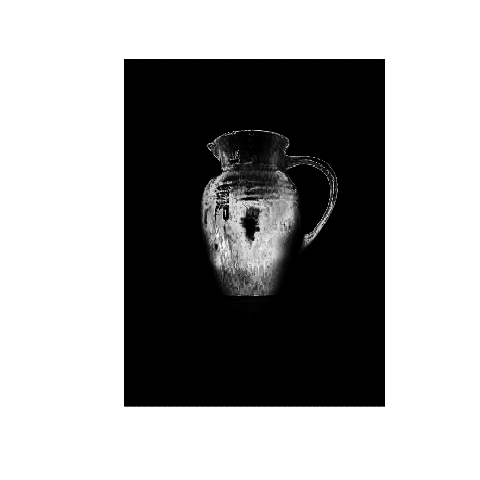
\includegraphics[width=0.49\textwidth]{pitcher}
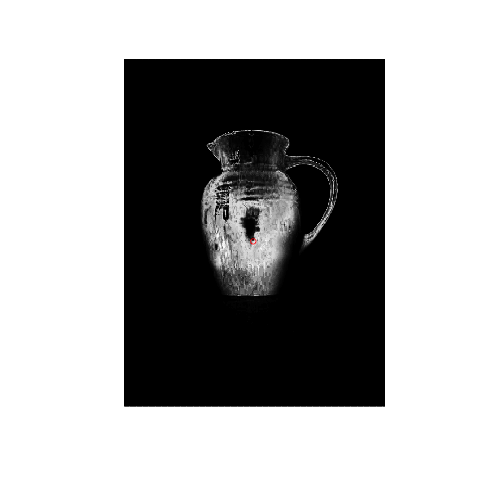
\includegraphics[width=0.49\textwidth]{centerOfMass}
\caption{ probability density of pitcher detection, along with its center of mass }
\label{pitcher}
\end{figure}
The pitcher is detected, and no pixels from outside the pitcher are picked up. Specular highlights present in the center of the image are not detected as they do not have the same color distribution as the training set --- the training set is mostly red, and the specular highlights are mostly white. 

\section*{Question 10}
The center of mass can be seen in figure \ref{pitcher} and the iso-probability curves along with the spatial covariance are shown in figure \ref{spat}. 

\begin{figure}[h!]
  \centering
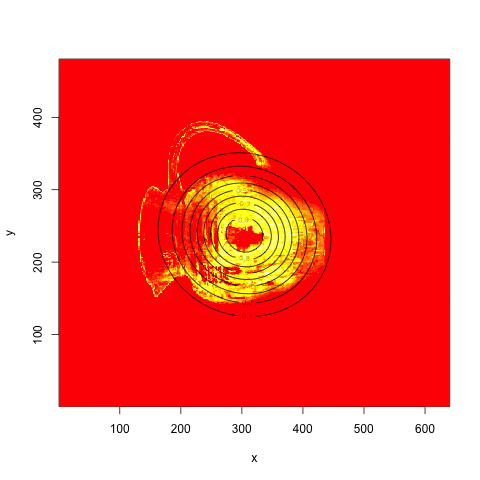
\includegraphics[width=0.45\textwidth]{spat}
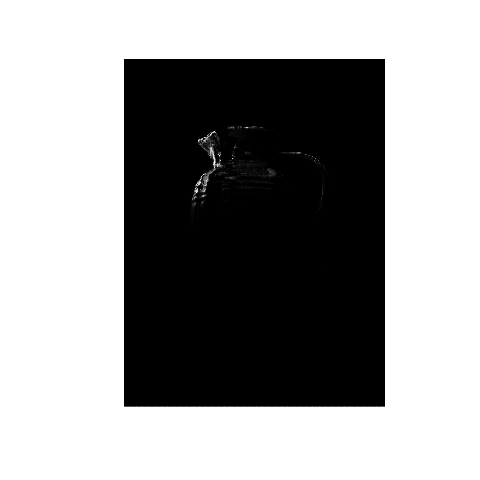
\includegraphics[width=0.45\textwidth]{newMap}
\caption{ iso-probability curves and 2-d probabilities for kande2.png}
\label{spat}
\end{figure}

\section*{Question 11}
We test our trained model on a different picture of a pitcher. We use the same training data, and display the probability that pixels from the new image are a part of the old distribution. We get the 2-d probability map shown in figure \ref{spat}. The results are poor, which is unsurprising as the pitcher appears as a significantly different shade of red under the different lighting conditions. 

